\chapter{Proportion / évolution}
\section{Proportion}
\begin{df}
	\ajusteliste
	\begin{wrapstuff}[r,width=6cm]
		\begin{center}
			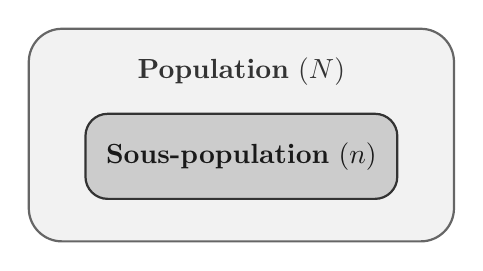
\begin{tikzpicture}[x=9mm,y=9mm]
				\draw[thick, fill=black!5, draw=black!60, rounded corners=12pt] (0,0) rectangle (6,3);
				\node[black!80] at (3, 2.4) {\textbf{Population} ($N$)};
				\draw[thick, fill=black!20, draw=black!80, rounded corners=8pt] (0.8,0.6) rectangle (5.2,1.8);
				\node[black!90] at (3, 1.2) {\textbf{Sous-population} ($n$)};
			\end{tikzpicture}
		\end{center}
		\vspace{-10mm}
	\end{wrapstuff}
	Soit $n$ l'effectif d'une sous-population incluse dans une population globale d'effectif $N$.

	La \textbf{proportion} $p$ de cette sous-population au sein de la population totale est donnée par :

	\cmath{p = \dfrac{n}{N}}
\end{df}

\begin{ex}
	\ajusteliste
	\begin{wrapstuff}[r,width=5cm]
		\begin{center}
			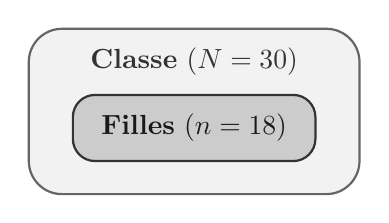
\begin{tikzpicture}[x=7mm,y=7mm]
				\draw[thick, fill=black!5, draw=black!60, rounded corners=12pt] (0,0) rectangle (6,3);
				\node[black!80] at (3, 2.4) {\textbf{Classe} ($N=30$)};
				\draw[thick, fill=black!20, draw=black!80, rounded corners=8pt] (0.8,0.6) rectangle (5.2,1.8);
				\node[black!90] at (3, 1.2) {\textbf{Filles} ($n=18$)};
			\end{tikzpicture}
		\end{center}
		\vspace{-15mm}
	\end{wrapstuff}
	Dans une classe de $30$ élèves, il y a $18$ filles.

	La proportion de filles dans cette classe est : $p = \dfrac{18}{30} = 0{,}6$ (soit $60$\%)
\end{ex}

\vspace{8mm}
\begin{prop}
	Une \textbf{proportion} s'exprime par un nombre compris entre $0$ et $1$ (soit entre $0\,\%$ et $100\,\%$). On a : \cmath{0 \leqslant p \leqslant 1}
\end{prop}

\begin{rmq}
	\ajusteliste
	\begin{itemize}
		\item La \textbf{proportion} est une valeur théorique ou fixe mesurée sur une population globale.
		\item La \textbf{fréquence} est le résultat d'une observation ou d'un comptage sur un échantillon donné (par exemple lors d'une expérience aléatoire ou d'un sondage).
	\end{itemize}
\end{rmq}

\begin{rmq}
	Pour retrouver les trois formules associées :
	\begin{wrapstuff}[r,width=7cm]
		\vspace{-5mm}
		\begin{center}
			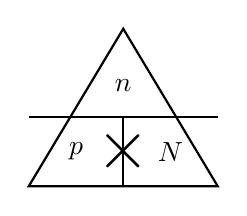
\begin{tikzpicture}[x=8mm,y=8mm]
				% Triangle principal
				\draw[thick] (0,0) -- (3,0) -- (1.5,2.5) -- cycle;
				\draw[thick] (0,1.1) -- (3,1.1);
				\draw[thick] (1.5,0) -- (1.5,1.1);
				% Labels
				\node at (1.5, 1.6) {\textbf{$n$}};
				\node at (0.75, 0.55) {\textbf{$p$}};
				\node at (2.25, 0.55) {\textbf{$N$}};
				\node at (1.5, 0.55) {\Huge$\times$};
			\end{tikzpicture}
		\end{center}
		\vspace{-10mm}
	\end{wrapstuff}
	\begin{itemize}
		\item \makebox[2cm][l]{$p = \dfrac{n}{N}$} pour calculer une proportion
		\item \makebox[2cm][l]{$n = p \times N$} pour calculer un effectif partiel
		\item \makebox[2cm][l]{$N = \dfrac{n}{p}$} pour retrouver l'effectif total
	\end{itemize}
\end{rmq}

\begin{ex}
	\ajusteliste
	\begin{enumerate}
		\item {Calculer une proportion}

		      Dans une entreprise de $250$ salariés, $65$ travaillent dans le service commercial.

		      \cmath{p = \dfrac{65}{250} = 0{,}26 \quad \text{soit } 26\,\%}

		      La proportion de salariés travaillant au service commercial est de $26\,\%$.

		\item {Calculer un effectif}

		      Dans un lycée de $1\,200$ élèves, $15\,\%$ des élèves sont inscrits en spécialité Mathématiques (soit $p = 0{,}15$).

		      \cmath{n = 0{,}15 \times 1\,200 = 180}

		      Il y a $180$ élèves inscrits en spécialité Mathématiques.
		\item {Retrouver l'effectif total}

		      Dans un club sportif, $42$ adhérents pratiquent le tennis, ce qui représente $35\,\%$ de l'effectif total du club (soit $p = 0{,}35$).

		      \cmath{N = \dfrac{42}{0{,}35} = 120}

		      Le club compte $120$ adhérents au total.
	\end{enumerate}
\end{ex}

\section{Proportion de proportion}
\begin{prop}
	\ajusteliste
	\begin{wrapstuff}[r,width=7.5cm]
		\begin{center}
			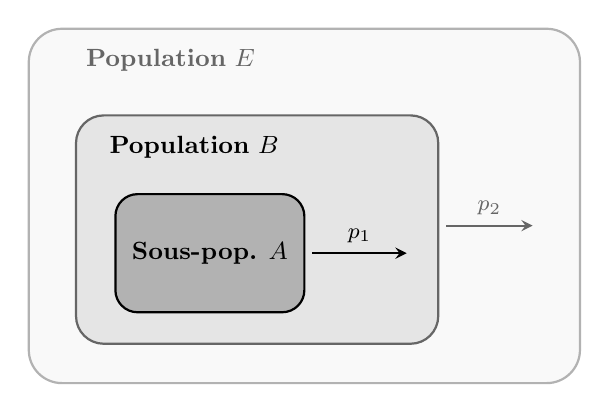
\begin{tikzpicture}[x=1cm, y=1cm]
				\draw[thick, fill=gray!5, draw=gray!60, rounded corners=12pt] (0,0) rectangle (7,4.5);
				\node[gray!80!black, font=\small] at (1.8, 4.1) {\textbf{Population} $E$};
				\draw[thick, fill=black!10, draw=black!60, rounded corners=10pt] (0.6,0.5) rectangle (5.2,3.4);
				\node[black!80!black, font=\small] at (2.1, 3) {\textbf{Population} $B$};
				\draw[thick, fill=black!30, draw=black!90!black, rounded corners=8pt] (1.1,0.9) rectangle (3.5,2.4);
				\node[black!90!black, font=\small] at (2.3, 1.65) {\textbf{Sous-pop.} $A$};
				\draw[->, >=stealth, thick, black!80!black] (3.6, 1.65) -- (4.8, 1.65) node[midway, above, font=\footnotesize] {$p_1$};
				\draw[->, >=stealth, thick, gray!80!black] (5.3, 2) -- (6.4, 2) node[midway, above, font=\footnotesize] {$p_2$};
			\end{tikzpicture}
			\vspace{-23mm}
		\end{center}
	\end{wrapstuff}

	Soit une sous-population $A$ incluse dans $B$, elle-même incluse dans une population $E$.

	Si $A$ a une proportion $p_1$ dans $B$, et $B$ a une proportion $p_2$ dans $E$, alors la proportion $p$ de $A$ dans $E$ est :

	\cmath{p = p_1 \times p_2}

\end{prop}

\vspace{12mm}

\begin{ex}
	Dans un lycée, $60\,\%$ des élèves sont en classe de Seconde (soit $p_1 = 0{,}6$).

	Parmi ces élèves de Seconde, $55\,\%$ étudient l'espagnol en LV2 (soit $p_2 = 0{,}55$).

	La proportion $p$ d'élèves de Seconde étudient l'espagnol dans l'ensemble du lycée est :

	\cmath{p = p_1 \times p_2 = 0{,}6 \times 0{,}55 = 0{,}33 \quad \text{(soit } 33\,\%\text{)}}

	Ainsi, $33\,\%$ des élèves du lycée sont des élèves de Seconde qui étudient l'espagnol.
\end{ex}

